%Umfrage
\section{Nutzerstudie}
Im Rahmen der Bedürfnisermittlung wurde eine Nutzerstudie durchgeführt. Im Rahmen einer Onlineumfrage wurden 170 Teilnehmer (Stand: 27.05.2020) zu ihren Präferenzen und Hauptinteressen befragt.
Um Teilnehmer für die Nutzerstudie zu gewinnen, wurde diese auf dem Sozialen Netzwerk \href{https://www.reddit.com/}{Reddit} und an private Kontakte verbreitet. Die Umfrage startete am 18.05.2020. Um Anreize für die Beteiligung an der Umfrage zu schaffen, wurde allen Teilnehmern die Teilnahme an der Verlosung eines Gutscheins für das Online-Warenhaus Amazon angeboten.
Die Anforderungen an \softwarename wurden aus der Umfrage abgeleitet, um den Anforderungen der Zielgruppe möglichst exakt zu entsprechen.
\\
Im folgenden werden die Ergebnisse vorgestellt.
Alle vorgestellten Ergebnisse beziehen sich auf den Stand der Studie am 27.05.2020

\subsection{Altersverteilung}
In der Umfrage wurde das Geburtsjahr der Teilnehmer abgefragt. Da sich unsere Zielgruppe auf Personen unter 35 fokussiert, trägt dies dazu bei, die Relevanz der Ergebnisse der Nutzerstudie besser einschätzen zu können.
\\
\begin{figure}[h]
    \centering
    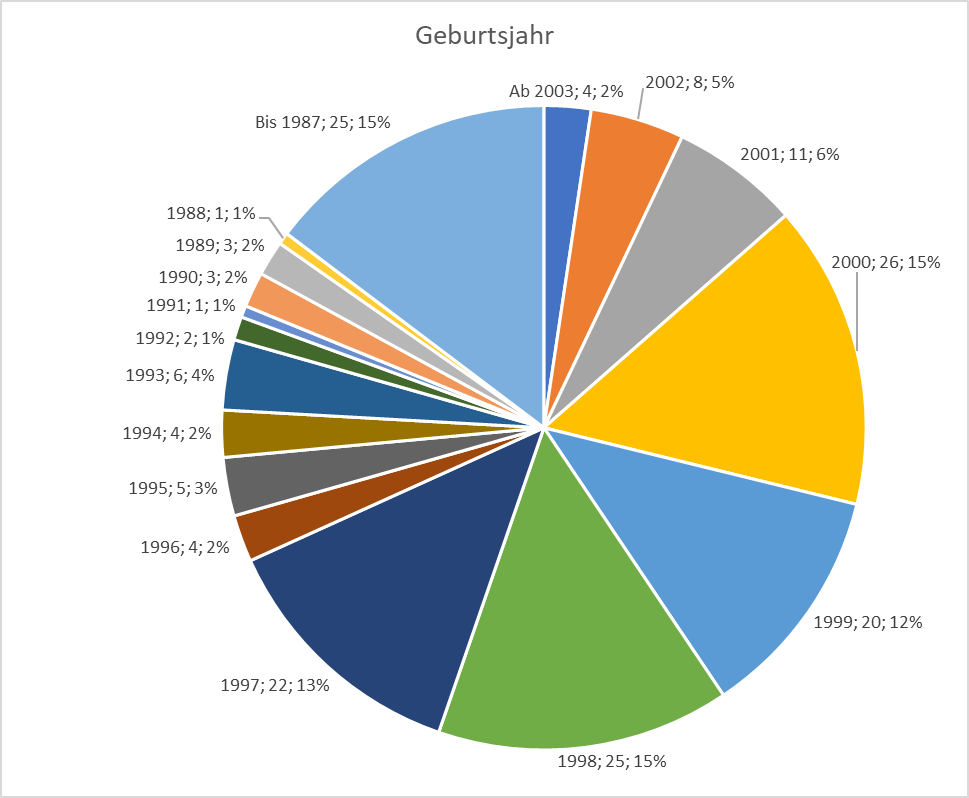
\includegraphics[width=0.7\textwidth]{media/diagram/geburtsjahr.png}
    \caption{Verteilung der Geburtsjahre der Befragten}
\end{figure}
\\
Es ist gut zu erkennen, dass das mittlere Alter der Befragten bei etwas über 20 Jahren liegt. Insgesamt haben hauptsächlich Personen zwischen 17 und 40 Jahren an der Umfrage teilgenommen.
Dies entspricht der angestrebten Zielgruppe.
\subsection{Selbsteinschätzung von Wissen und Interesse am Thema Luftverschmutzung}
Für eine Beurteilung des Interesses an den in \softwarename gezeigten Informationen wurde nach dem Interesse auf der Seite der Nutzer gefragt.
Um abzuschätzen wie viel Wissen bereits über \gls{Luftverschmutzung} vorhanden ist wurde gefragt, wie die Nutzer ihr eigenes Wissen über \gls{Luftverschmutzung} einschätzen.
\\
Bei beiden Einschätzungen wurde eine Skala von 1 bis 5 verwendet, wobei 1 für \enquote{Sehr wichtig} und 5 für \enquote{Sehr unwichtig} steht.
\\
\begin{figure}[h]
    \begin{subfigure}[c]{0.49\textwidth}
        \centering        
        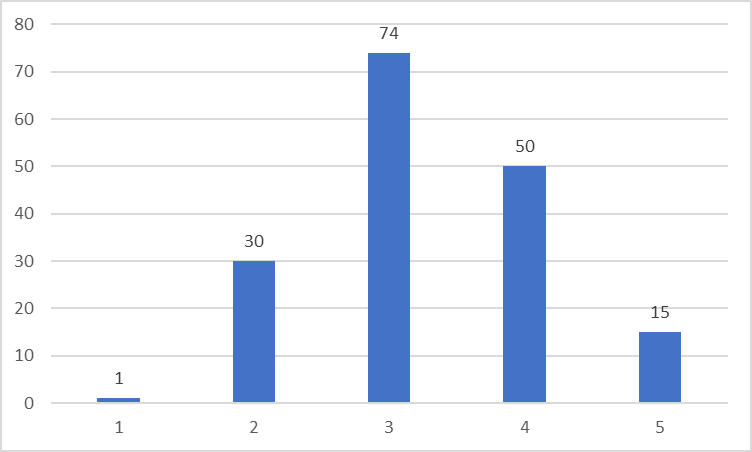
\includegraphics[scale=0.2]{media/diagram/eigenesWissen.png}
        \subcaption{Einschätzung zum eigenen Wissen über Luftverschmutzung}
    \end{subfigure}
    \begin{subfigure}[c]{0.49\textwidth}
        \centering        
        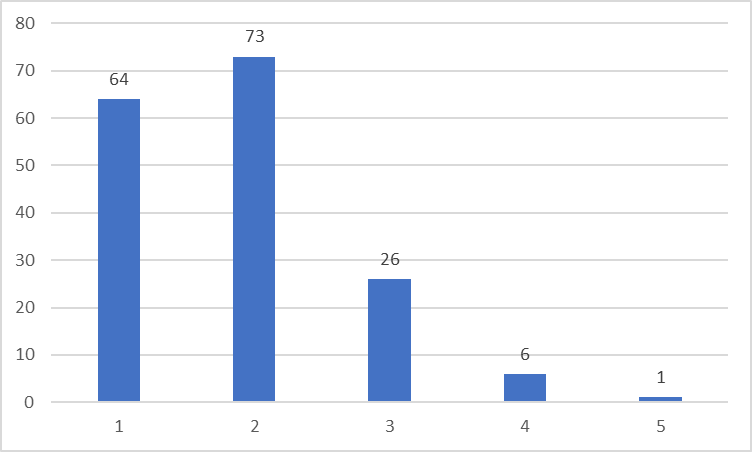
\includegraphics[scale=0.2]{media/diagram/WichtigkeitVonInfos.png}
        \subcaption{Einschätzung zur Wichtigkeit von Informationen über Luftverschmutzung}
    \end{subfigure}
    \caption{Selbsteinschätzung der Nutzer}
\end{figure}
\\
Weiter wurden die Nutzer gefragt wie sie ihre Informationen zum Thema \gls{Luftverschmutzung} erhalten. Die verbreitetsten Informationsquellen sind hierbei
\begin{itemize} [noitemsep]
    \item Nachrichtensendungen und Berichterstattungen (circa 79\%)
    \item Informationen aus dem Internet (circa 78 \%)
    \item Gespräche mit anderen Personen (circa 26 \%)
\end{itemize}
Daraus ergibt sich, dass eine Webseite für die Vermittlung gut geeignet ist, da dieses Medium bereits weit verbreitet ist.

\subsection{Einschätzung zu Aufrufen der Webseite}
Die Teilnehmer wurden gefragt wie oft sie eine Webseite mit \gls{Luftqualitaetsdaten} aufrufen würden.
\\
\begin{figure}[h]
    \centering
    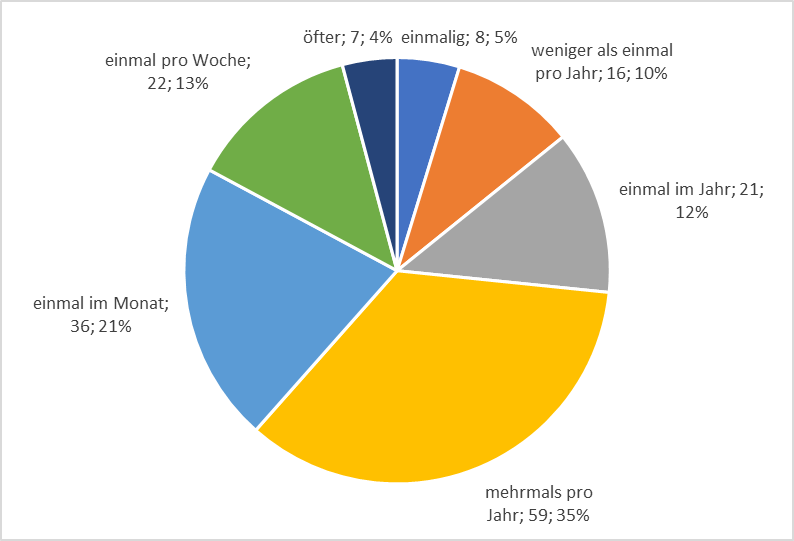
\includegraphics[width=0.7\textwidth]{media/diagram/aufrufe.png}
    \caption{Geschätzte Häufigkeit der Aufrufe}
\end{figure}
\\
Dieser Parameter ist hilfreich um die Last auf die Webseite abzuschätzen.
Es ist gut zu erkenne, dass die meisten Nutzer die Webseite zwischen mehrmals in einem Jahr auf rufen würden.
Dementsprechend muss \softwarename diese Last bewältigen können.
\\
Die häufigsten Gründe für den Aufruf einer solchen Webseite sind laut der Nutzerstudie
\begin{itemize} [noitemsep]
    \item Information vor Schul- oder Hausarbeiten
    \item Generelles Interesse
    \item Verifikation von Gerüchten
    \item Vor Reisen oder Wohnortswechsel
\end{itemize}
Die Geräte von welchen die Webseite im wesentlichen aufgerufen wird sind.
\begin{itemize} [noitemsep]
    \item Smartphones
    \item Tablets
    \item PCs
    \item Laptops
\end{itemize}

\subsection{Art des Informationsbedürfnisses}
Das Interesse an \gls{Luftverschmutzung} in Abhängigkeit von der räumlichen Nähe zum Nutzer, wurde ebenfalls befragt.
Viele Teilnehmer der Studie interessieren sich primär für die Verschmutzung der Luft in ihrer eigenen Region. Viele Befragte hielten auch einen Überblick über \gls{Luftverschmutzung} in Deutschland für wichtig. Für die Verschmutzung der Luft in anderen Regionen zeigte sich hingegen ein geringeres Interesse.
\\
\begin{figure}[h]
    \centering
    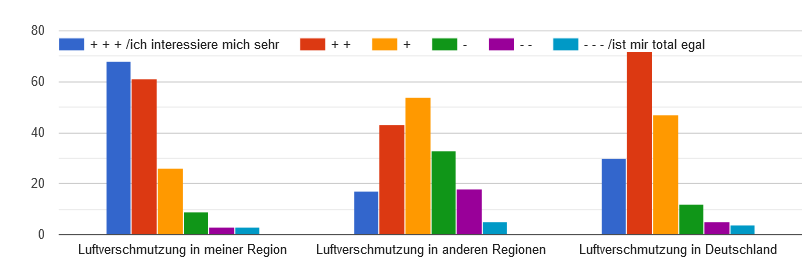
\includegraphics[width=1\textwidth]{media/diagram/interesse.png}
    \caption{Interesse der Nutzer an der Luftverschmutzung in verschiedenen Regionen}
\end{figure}
\\
Weiter gaben die Teilnehmer an,  dass sowohl die Auswirkungen und Ursachen von \gls{Luftverschmutzung} sehr wichtig sind. Eher weniger wichtig sind die Messmethoden der Luftverschmutzung
\\
\begin{figure}[h]
    \centering
    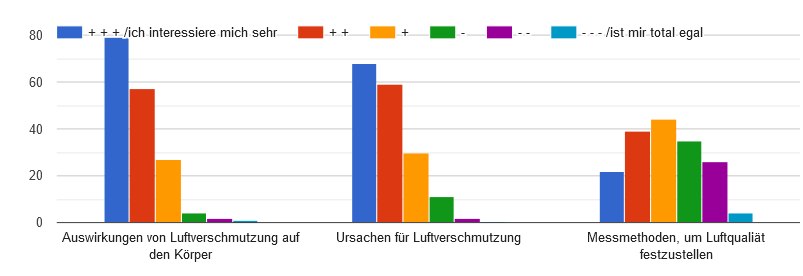
\includegraphics[width=1\textwidth]{media/diagram/interesse2.png}
    \caption{Interesse der Nutzer an Zusatzinformationen zu Luftverschmutzung}
\end{figure}
\\
Auch ergab sich, dass sowohl die zeitliche Entwicklung der Luftqualitätsdaten als auch die momentane Luftqualität etwa gleich wichtig für unsere Zielgruppe sind. Interesse am Bau von \gls{DIY}-\glspl{Sensor} zeigen etwa 40\%  der Teilnehmer.
Über die Hälfte der Studien-teilnehmer gab an, dass die Vergleiche von regionaler \gls{Luftverschmutzung} mit der Belastung der Luft durch einzelne technische Geräte sehr hilfreich finden würden.
\\
Als besonders wichtig hoben viele Teilnehmer die Übersichtlichkeit und die Benutzbarkeit für Laien hervor.

\subsection{Darstellungsweisen von Luftverschmutzung}
Da die Darstellungsform einen sehr direkten Einfluss auf die Benutzerfreundlichkeit hat, haben wir diese als zusätzliche Frage aufgegriffen.
\\
\begin{figure}[h]
    \centering
    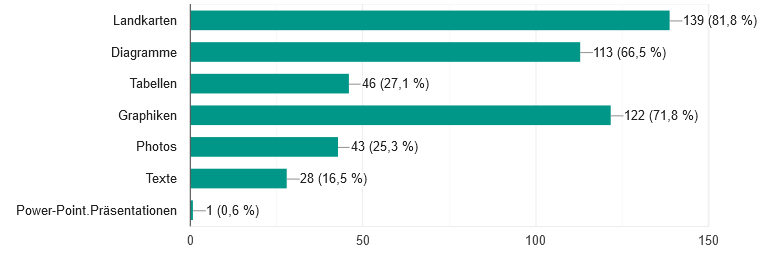
\includegraphics[width=1\textwidth]{media/diagram/darstellung.png}
    \caption{Präferenzen bei der Darstellung von Luftverschmutzung}
\end{figure}
\\
Gut zu erkennen ist hier das gerade die Darstellung als Karte von einer großen Anzahl Teilnehmer als hilfreich empfunden wird.
Graphiken und Diagramme sind auch gerne gesehen, während Tabellen oder sachliche Texte als weniger hilfreich empfunden werden.

\subsection{Allgemeine Anregungen}
Die Umfrage beinhaltete auch mehrere Fragen, die sich mit allgemeinen Anregungen zum Projekt befassten. Eine Auswahl der abgegebenen Anregung sieht wie folgt aus:
\begin{itemize} [noitemsep]
    \item Anzeigen der lokal-geltenden Grenzwerte
    \item Messwerten übersichtlich mit einer konkreten bedeutung versehen
    \item Standort und qualität der Sensoren beschreiben
    \item Farbige Kennzeichnung kritischer Werte
\end{itemize}
Leider sind nicht alle abgegebene Anregungen umsetzbar, da die Daten hierzu nicht zwingend vorliegen oder eine Umsetzung die Daten zu sehr vereinfachen würde. Die obige Auflistung zeigt deshalb lediglich die umsetzbaren Anregungen auf